\chapter{EUTRO Module}

The EUTRO module describes the oxygenation of a river.
It is not restricted to modeling reaeration and the global oxidizable load.
It also takes into account the effect of planktonic photosynthesis,
and furthermore models the nitric and phosphoric nutrients and their effect
on phytoplankton (\cite{gosse_doubs_1989} and \cite{gosse_doubs_1983}).\\

This module looks like a combination of the O$_2$ and BIOMASS modules,
except for a more precise treatment of some parameters,
taking into account of the ammonia load in exchanges between nitrogen and phytoplankton,
and of phytoplankton in the calculation of photosynthesis.
More sophisticated than the O$_2$ module, EUTRO requires setting the values of
28 parameters (excluding parameterizing the weirs).\\

It involves 8 tracers:

\begin{itemize}
\item dissolved oxygen O$_2$,
\item phytoplankton biomass (which consumes oxygen through photosynthesis) PHY,
\item the main elements that influence their production
  (phosphorus, nitrogen, ammonia load, organic load)
  as well as the mineral forms associated with phosphorus and nitrogen:
\begin{itemize}
\item dissolved mineral phosphorus assimilable by phytoplankton PO$_4$,
\item degradable phosphorus non-assimilable by phytoplankton POR,
\item dissolved mineral nitrogen assimilable by phytoplankton NO$_3$,
\item ammonia load assimilable by phytoplankton (and consuming oxygen) NH$_4$,
\item degradable nitrogen non-assimilable by phytoplankton NOR,
\item organic load (consuming oxygen) L.
\end{itemize}
\end{itemize}


These variables are expressed in mg/l, except for biomass which is expressed in $\mu$g (Chlorophyll a)/l.\\

The hypothesis assumes these substances to act as tracers,
i.e. they are carried and dispersed in the mass of water.
In addition, they react with each other through biochemical processes.

\section{Processes represented}

Figure \ref{ecosyst_scheme} succinctly presents phenomena modeled\ by the EUTRO model.\\

The following parts show the parameters used and detail internal sources for each of the 8 tracers studied.\\

As with the BIOMASS model, the bottom and the processes which take place there are not modeled in the EUTRO model
(only a deposition flux is taken into account and the quantities deposited no longer appear in the equations).\\

\begin{figure}[H]
  \centering
%  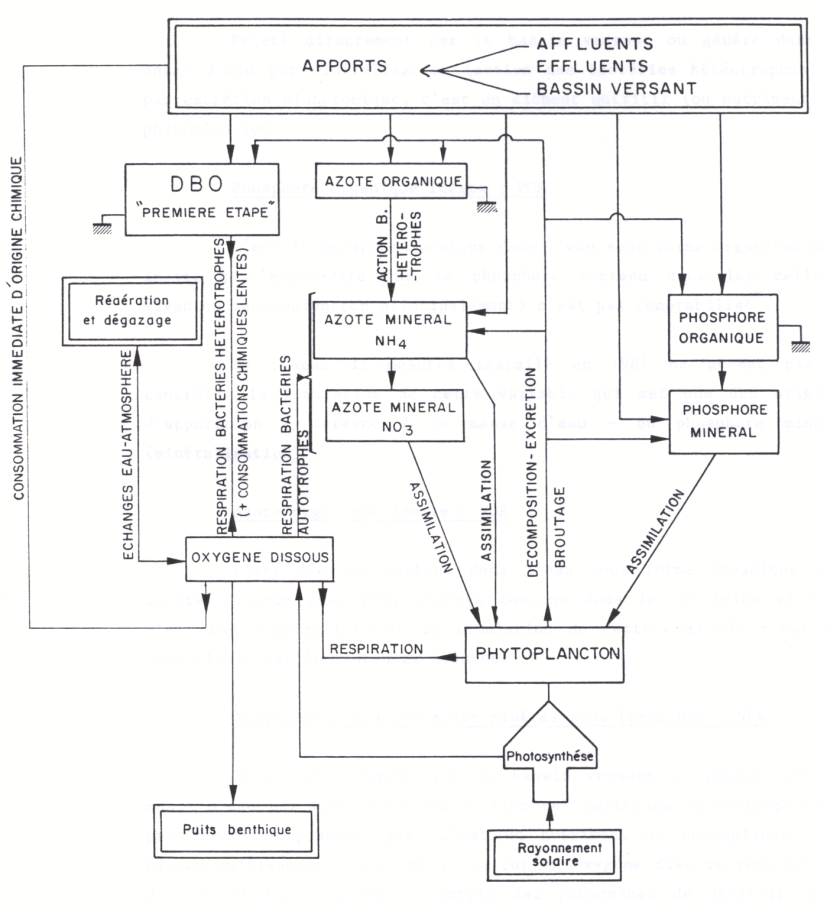
\includegraphics[scale=1.]{graphics/image38.png}
  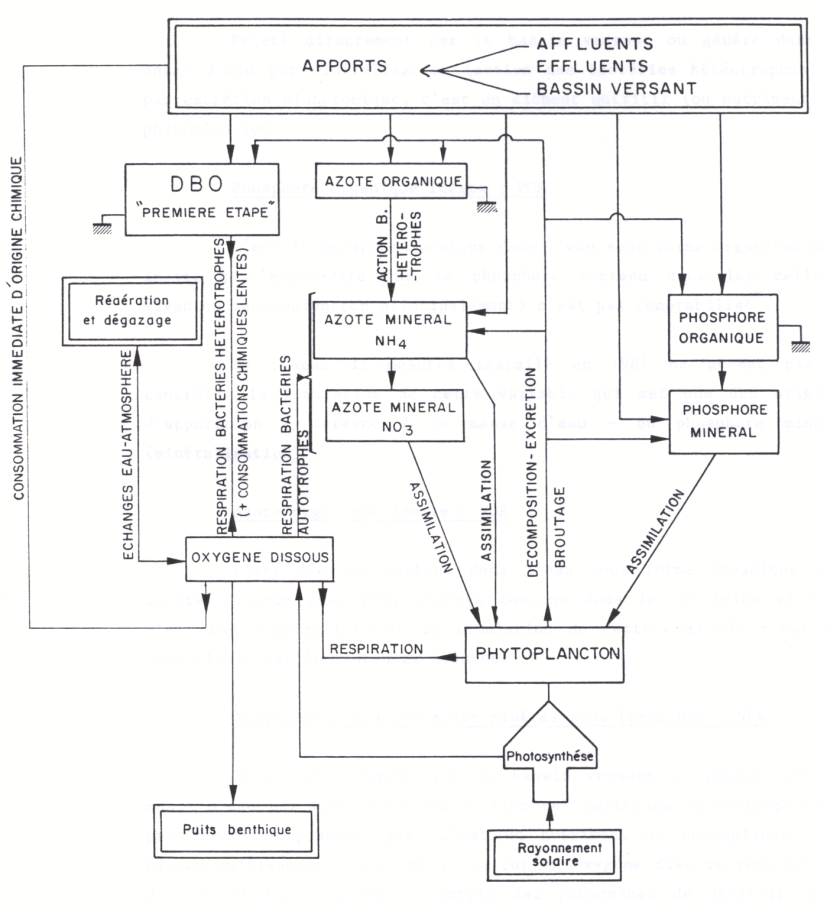
\includegraphics[width=3.76in,height=4.01in]{graphics/image38.png}
  \caption{Schematic representation of the ecosystem modeled by the EUTRO module \cite{gosse_doubs_1989}.
    Figure taken from \cite{elkadi_tracer_2012}.}
  \label{ecosyst_scheme}
\end{figure}

\section{Phytoplankton}

\subsection{Algal growth}

The rate of algal growth $CP$ (d$^{-1}$) is given by the equation:

\begin{equation}
  CP = C_{max} RAY g_1 LNUT \alpha_1.
\end{equation}

The parameters $C_{max}$, $RAY$, $g_1$ and $\alpha_1$ are defined in the same way as in the BIOMASS module.\\

On the other hand, the parameter representing the effects of phosphoric
and nitric nutrients on the algal growth $LNUT$ now takes into account
the ammonia load assimilable by the phytoplankton NH$_4$ and is therefore defined by:

\begin{equation}
  LNUT = \min \left( \frac{[PO_4]}{KP+[PO_4]}, \frac{[NO_3]+[NH_4]}{KN+[NO_3]+[NH_4]} \right),
\end{equation}

with $KP$ the constant of half-saturation in phosphate (mg/l) (about 0.005 mgP/l),
and $KN$ the constant of half-saturation in nitrates (mg/l) (about 0.03 mgN/l).\\

Note: The influence of nutrients on phytoplankton growth PHY is only an intermediate factor limiting $LNUT$.
When [PO$_4$] and [NO$_3$] are big enough, $LNUT$ is close to 1
and phytoplankton evolution no longer depends on nutrients.
In this case, there is no need to model the cycles of phosphorus and
nitrogen in order to simulate the evolution of phytoplankton.

\subsection{Algal disappearance}

The rate of algal disappearance $DP$ (d$^{-1}$) is given by the equation:

\begin{equation}
  DP = (RP + MP) g_2,
\end{equation}

where $RP$ and $MP$ are defined as in the BIOMASS module.
On the other hand, the effect of temperature on algal disappearance
is now represented by the function $g_2$ such that: $g_2 = (1,050)^{T-20}$,
where $T$ is the water temperature ($^{\circ}$C) (valid for 5$^{\circ}$C < $T$ < 25$^{\circ}$C).

\section{Nitric and phosphoric nutrients}

The following physical and biochemical parameters are used to describe processes
influencing the evolution of nitric and phosphoric nutrients:

\begin{itemize}
\item $fp$: average proportion of phosphorus in the cells of living phytoplankton (mgP/$\mu$ChlA),
\item $dtp$: proportion of directly assimilable phosphorus in dead phytoplankton ($\%$),
\item $k_{320}$: rate of transformation of POR into PO$_4$ through bacterial mineralization
  at 20$^{\circ}$C (d$^{-1}$),
\item $k_{620}$: rate of transformation of NOR into NO$_3$ through heterotrophic and autotrophic
  bacterial mineralization at 20$^{\circ}$C (d$^{-1}$),
\item $fn$: average proportion of nitrogen in the cells of living phytoplankton (mgN/$\mu$ChlA),
\item $dtn$: proportion of directly assimilable nitrogen in dead phytoplankton ($\%$),
\item $n$: quantity of oxygen consumed by nitrification (mgO$_2$/mgNH$_4$),
\item $k_{520}$: kinetics of nitrification at 20$^{\circ}$C (d$^{-1}$),
\item $F_{POR}$: deposition flux of non-algal organic phosphorus (g/m$^2$s) = W$_{POR}$.[POR],
  with W$_{POR}$ the sedimentation velocity of non-algal organic phosphorus (m/s),
\item $F_{NOR}$: deposition flux of non-algal organic nitrogen (g/m$^2$s) = W$_{NOR}$.[NOR],
  with W$_{NOR}$ the sedimentation velocity of non-algal organic nitrogen (m/s),
\item $Rn$: proportion of nitrogen assimilated in the form of NH$_4$ = $\frac{[NH_4]}{[NH_4]+[NO_3]}$.
\end{itemize}

\section{Organic load}

The following physical and biochemical parameters are used to describe processes
influencing the evolution of the organic load ($L$):

\begin{itemize}
\item $k_{120}$: constant of the kinetic degradation of the organic load at 20$^{\circ}$C (d$^{-1}$),
\item $g_3$: effect of temperature on degradation of the organic load = $(1.047)^{T-20}$,
  where $T$ is the water temperature ($^{\circ}$C) (valid for 5$^{\circ}$C < $T$ < 25$^{\circ}$C),
\item $F_{LOR}$: deposition flux of the organic load (g/m$^2$s) = $W_{LOR}$.[L],
  with $W_{LOR}$ the sedimentation velocity of the organic load (m/s).
\end{itemize}

\section{Dissolved oxygen}

The following physical and biochemical parameters are used to describe processes
influencing the dissolved oxygen balance (O$_2$):

\begin{itemize}
\item $f$: quantity of oxygen produced by photosynthesis (mgO$_2$/$\mu$gChlA),
\item $BEN$: benthic oxygen demand (gO$_2$/m$^2$/d) (cf. O$_2$ model),
\item $k_2$: coefficient of water-atmosphere gaseous exchange,
  also called coefficient of reaeration, at 20$^{\circ}$C (d$^{-1}$).
  It can be provided by the user or calculated using formulae in the literature (cf. O$_2$ module),
\item $g_4$: effect of temperature on natural reaeration = $(1.025)^{T-20}$,
  where $T$ is the water temperature ($^{\circ}$C) (valid for 5$^{\circ}$C < $T$ < 25$^{\circ}$C),
\item $C_s$: concentration of oxygen saturation in water (mgO$_2$/l).
  It can be determined from the water temperature (cf. O$_2$ module).
%\item $r$: relationship defining the influence of weirs on oxygen concentration (cf. O$_2$ module)
\end{itemize}

\section{Solved equations}

Equations of the EUTRO model are described below:\\

Tracer $\#$1: phytoplankton biomass

\begin{equation}
  F([PHY]) = (CP-DP) [PHY].
\end{equation}

Tracer $\#$2: assimilable mineral phosphorus

\begin{equation}
  F([PO_4]) = fp(dtp DP - CP) [PHY] + k_{320} g_2 [POR].
\end{equation}

Tracer $\#$3: non-assimilable phosphorus

\begin{equation}
  F([POR]) = fp(1-dtp) DP [PHY] - k_{320} g_2 [POR] - \frac{F_{POR}}{h}.
\end{equation}

Tracer $\#$4: assimilable mineral nitrogen

\begin{equation}
  F([NO_3]) = - fn (1- Rn) CP [PHY] + k_{520} g_2 [NH_4].
\end{equation}

Tracer $\#$5: non-assimilable nitrogen

\begin{equation}
  F([NOR]) = fn (1- dtn) DP [PHY] - k_{620} g_2 [NOR] - \frac{F_{NOR}}{h}.
\end{equation}

Tracer $\#$6: ammonia load

\begin{equation}
  F([NH_4]) = fn (dtn DP - Rn CP) [PHY] + k_{620} g_2 [NOR] - k_{520} g_2 [NH_4].
\end{equation}

Tracer $\#$7: organic load

\begin{equation}
  F([L]) = f.MP [PHY] - k_{120} g_3 [L] - \frac{F_{LOR}}{h}.
\end{equation}

Tracer $\#$8: dissolved oxygen

\begin{equation}
  F([O_2]) = f (CP - RP.g_1) [PHY] - n k_{520} g_2 [NH_4] - k_{120} g_3 [L] + k_2 g_4 (C_s - [O_2]) - \frac{BEN}{h}.
\end{equation}

Using the terminology and notations of section \ref{waq_models} and by setting:
$C_1$ = [PHY], $C_2$  = [PO$_4$], $C_3$ = [POR], $C_4$ = [NO$_3$], $C_5$ = [NOR],
$C_6$ = [NH$_4$], $C_7$ = [L], and $C_8$ = [O$_2$],
the matrices (8 $\times$ 8) $[\lambda]$ and $[\mu]$ containing the coefficients
$\lambda_i^j$ and $\mu_i^j$ are written as (only non-zero terms are mentioned):\\

$$  \lambda_i^j = \frac{1}{86400}
  \begin{pmatrix}
    CP-DP               & 0 &            0 & 0 & 0 & 0 & 0 & 0 \\
    fp (dtp DP -CP)     & 0 &  k_{320} g_2  & 0 & 0 & 0 & 0 & 0 \\
    fp (1-dtp) DP       & 0 & -k_{320} g_2  & 0 & 0 & 0 & 0 & 0 \\
   -fn (1 -Rn) CP       & 0 &        0 & 0 & 0 &  k_{520} g_2 & 0 & 0 \\
    fn (1-dtn) DP       & 0 &        0 & 0 & -k_{620} g_2 & 0 & 0 & 0 \\
    fn (dtn DP - Rn CP) & 0 &        0 & 0 &  k_{620} g_2 & -k_{520} g_2 & 0 & 0 \\
    f . MP              & 0 &        0 & 0 & 0 & 0 & -k_{120} g_3 & 0 \\
    f (CP - RP .  g_1 ) & 0 &        0 & 0 & 0 & -n.k_{520} g_2 & -k_{120} g_3 & - k_2 g_4
  \end{pmatrix}
$$  

$$
  \mu_i^j = 
  \begin{pmatrix}
   0 & 0 & 0 & 0 & 0 & 0 & 0 & 0 \\
   0 & 0 & 0 & 0 & 0 & 0 & 0 & 0 \\
   0 & 0 & -W_{POR} & 0 & 0 & 0 & 0 & 0 \\
   0 & 0 & 0 & 0 & 0 & 0 & 0 & 0 \\
   0 & 0 & 0 & 0 & -W_{NOR} & 0 & 0 & 0 \\
   0 & 0 & 0 & 0 & 0 & 0 & 0 & 0 \\
   0 & 0 & 0 & 0 & 0 & 0 & -W_{LOR} & 0 \\
   0 & 0 & 0 & 0 & 0 & 0 & 0 & 0 
  \end{pmatrix}
$$

The only non-zero terms $\lambda_i^0$ and $\mu_i^0$ are:\\

$\lambda_8^0 = \frac{k_2 g_4 C_s}{86400}$ ; $\mu_8^0 = -\frac{BEN}{86400}$

Divisions by 86,400 are performed to scale down time to one second.
